\documentclass[UTF8]{ctexart}
\usepackage[left=2cm,right=2cm,top=1.5cm,bottom=1.5cm]{geometry}
\usepackage{tikz}
\usepackage{tikz-network}
\usepackage{amsmath}

\begin{document}
	\title{编译原理 HW2}
	\author{肖桐 PB18000037}
	\date{2020 年 9 月 26 日}
	\maketitle
	
	\noindent
	NFA:\newline
	由$(a|b)^*$可以知道, 处于开始状态时, 遇到任意个$a, b$均可继续保持在开始状态, 因此开始状态需要两个指向自己的箭头. 同时因为$abb$的存在, 开始状态还需要能够接受字符流$abb$之后进入接收状态. 进入接收状态之后, 不论再接收到多少个$a, b$都仍然处在接收状态. 即可得到以下NFA:(图中用绿色顶点表示接收状态, 同时因为要显示出 start 的箭头, 不得不加上最开始的顶点 i, 可忽略)\newline
	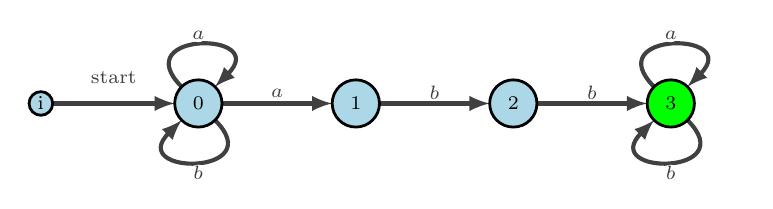
\begin{tikzpicture}
		\Vertex[label = i, size = 0.3]{Start}
		\Vertex[label = 0, x = 2]{0}
		\Vertex[label = 1, x = 4]{1}
		\Vertex[label = 2, x = 6]{2}
		\Vertex[label = 3, x = 8, color = green]{3}
		\Edge[Direct, label = start, position = above](Start)(0)
		\Edge[Direct, label = $a$, position = above, loopposition = 90](0)(0)
		\Edge[Direct, label = $b$, position = below, loopposition = -90](0)(0)
		\Edge[Direct, label = $a$, position = above](0)(1)
		\Edge[Direct, label = $b$, position = above](1)(2)
		\Edge[Direct, label = $b$, position = above](2)(3)
		\Edge[Direct, label = $a$, position = above, loopposition = 90](3)(3)
		\Edge[Direct, label = $b$, position = below, loopposition = -90](3)(3)
	\end{tikzpicture}\newline
	DFA:\newline
	因为DFA要求每个状态经一个字符后只能到达一个状态, 因此在原NFA中, 状态$0$需要减少一个带$a$的箭头. 显然经$a$到达状态$1$的箭头不能减去, 否则无法到达接收状态, 因此删去指向状态$0$自身的带$a$箭头.\newline
	同时状态$1$缺少一个带$a$的箭头, 对正则表达式分析知, 接受任意个$a$(至少有一个)与接受$1$个字符$a$对于正则表达式而言是等价的, 因此从状态$1$引出的带$a$的箭头应指向$1$自身.\newline
	同样的, 状态$2$也缺少一个带$a$的箭头, 对正则表达式分析知, 再识别字符串$ab$之后若再遇到字符$a$, 则字符串$ab$只能算作是满足正则表达式$(a|b)^*$的字符串, 而不是满足正则表达式$abb$的字符串, 因此此时与仅识别了字符串$a$是等价的, 因此从$2$引出的带$a$箭头应当指向状态$1$, 故可得到以下的DFA:\newline
	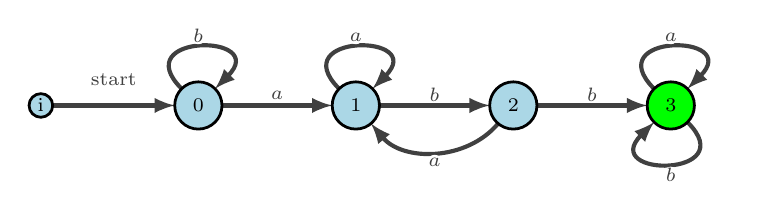
\begin{tikzpicture}
		\Vertex[label = i, size = 0.3]{Start}
		\Vertex[label = 0, x = 2]{0}
		\Vertex[label = 1, x = 4]{1}
		\Vertex[label = 2, x = 6]{2}
		\Vertex[label = 3, x = 8, color = green]{3}
		\Edge[Direct, label = start, position = above](Start)(0)
		\Edge[Direct, label = $b$, position = above, loopposition = 90](0)(0)
		\Edge[Direct, label = $a$, position = above](0)(1)
		\Edge[Direct, label = $a$, position = above, loopposition = 90](1)(1)
		\Edge[Direct, label = $b$, position = above](1)(2)
		\Edge[Direct, label = $a$, position = below, bend = 50](2)(1)
		\Edge[Direct, label = $b$, position = above](2)(3)
		\Edge[Direct, label = $a$, position = above, loopposition = 90](3)(3)
		\Edge[Direct, label = $b$, position = below, loopposition = -90](3)(3)
	\end{tikzpicture}
	\newline
	按算法, 由正则表达式$(a|b)^*abb(a|b)^*$得到的NFA:\newline
	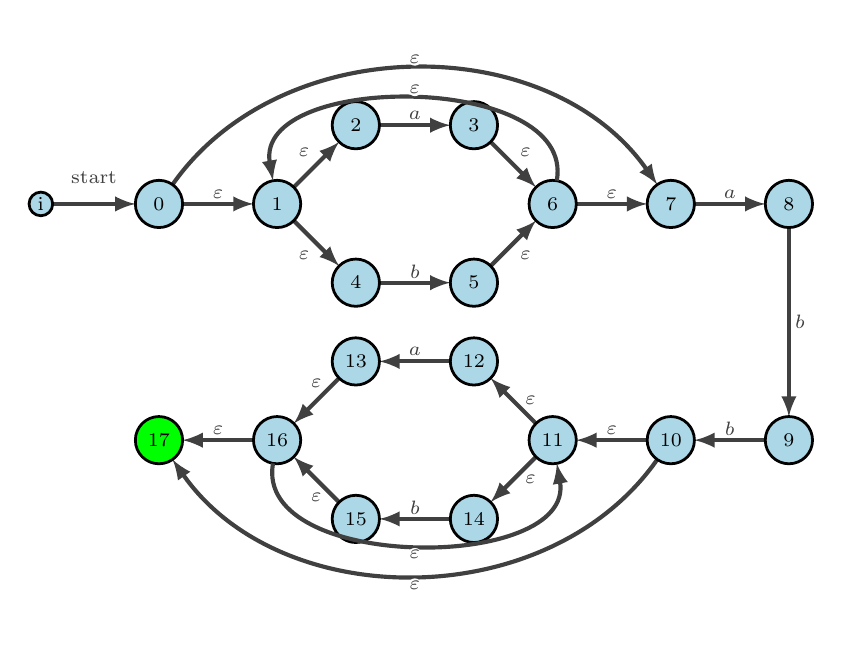
\begin{tikzpicture}
		\Vertex[label = i, size = 0.3]{Start}
		\Vertex[label = 0, x = 1.5]{0}
		\Vertex[label = 1, x = 3]{1}
		\Vertex[label = 2, x = 4, y = 1]{2}
		\Vertex[label = 3, x = 5.5, y = 1]{3}
		\Vertex[label = 4, x = 4, y = -1]{4}
		\Vertex[label = 5, x = 5.5, y = -1]{5}
		\Vertex[label = 6, x = 6.5]{6}
		\Vertex[label = 7, x = 8]{7}
		\Vertex[label = 8, x = 9.5]{8}
		\Vertex[label = 9, x = 9.5, y = -3]{9}
		\Vertex[label = 10, x = 8, y = -3]{10}
		\Vertex[label = 11, x = 6.5, y = -3]{11}
		\Vertex[label = 12, x = 5.5, y = -2]{12}
		\Vertex[label = 13, x = 4, y = -2]{13}
		\Vertex[label = 14, x = 5.5, y = -4]{14}
		\Vertex[label = 15, x = 4, y = -4]{15}
		\Vertex[label = 16, x = 3, y = -3]{16}
		\Vertex[label = 17, x = 1.5, y = -3, color = green]{17}
		\Edge[Direct, label = start, position = above](Start)(0)
		\Edge[Direct, label = $\varepsilon$, position = above](0)(1)
		\Edge[Direct, label = $\varepsilon$, position = {above left=1mm}](1)(2)
		\Edge[Direct, label = $\varepsilon$, position = {below left=1mm}](1)(4)
		\Edge[Direct, label = $a$, position = above](2)(3)
		\Edge[Direct, label = $b$, position = above](4)(5)
		\Edge[Direct, label = $\varepsilon$, position = {above right=1mm}](3)(6)
		\Edge[Direct, label = $\varepsilon$, position = {below right=1mm}](5)(6)
		\Edge[Direct, label = $\varepsilon$, position = above, bend = -100, NotInBG](6)(1)
		\Edge[Direct, label = $\varepsilon$, position = above, bend = 55](0)(7)
		\Edge[Direct, label = $\varepsilon$, position = above](6)(7)
		\Edge[Direct, label = $a$, position = above](7)(8)
		\Edge[Direct, label = $b$, position = right](8)(9)
		\Edge[Direct, label = $b$, position = above](9)(10)
		\Edge[Direct, label = $\varepsilon$, position = above](10)(11)
		\Edge[Direct, label = $\varepsilon$, position = {above, right=1mm}](11)(12)
		\Edge[Direct, label = $a$, position = above](12)(13)
		\Edge[Direct, label = $\varepsilon$, position = {below, right=1mm}](11)(14)
		\Edge[Direct, label = $b$, position = above](14)(15)
		\Edge[Direct, label = $\varepsilon$, position = {above=1mm}](13)(16)
		\Edge[Direct, label = $\varepsilon$, position = {below=1mm}](15)(16)
		\Edge[Direct, label = $\varepsilon$, position = above](16)(17)
		\Edge[Direct, label = $\varepsilon$, position = below, bend = -100, NotInBG](16)(11)
		\Edge[Direct, label = $\varepsilon$, position = below, bend = 55](10)(17)
	\end{tikzpicture}\newline
	下面用子集构造法求出该NFA对应的DFA(不一定最简).\newline
	记初始状态$0$的$\varepsilon$-闭包为$A = \{0, 1, 2, 4, 7\}$.\newline
	若集合$T$为从状态集合$A$中的某一状态$s$出发, 通过字符$a, \varepsilon$转换可以到达的NFA状态组成的集合, 则记$A\stackrel{a}{\longrightarrow}T$.
	$A\stackrel{a}{\longrightarrow}\{1, 2, 3, 4, 6, 7, 8\} = B$\newline
	$A\stackrel{b}{\longrightarrow}\{1, 2, 4, 5, 6, 7\} = C$\newline
	$B\stackrel{a}{\longrightarrow}\{1, 2, 3, 4, 6, 7, 8\} = B$\newline
	$B\stackrel{b}{\longrightarrow}\{1, 2, 4, 5, 6, 7, 9\} = D$\newline
	$C\stackrel{a}{\longrightarrow}\{1, 2, 3, 4, 6, 7, 8\} = B$\newline
	$C\stackrel{b}{\longrightarrow}\{1, 2, 4, 5, 6, 7\} = C$\newline
	$D\stackrel{a}{\longrightarrow}\{1, 2, 3, 4, 6, 7, 8\} = B$\newline
	$D\stackrel{b}{\longrightarrow}\{1, 2, 4, 5, 6, 7, 10, 11, 12, 17\} = E$\newline
	$E\stackrel{a}{\longrightarrow}\{1, 2, 3, 4, 6, 7, 8, 11, 12, 13, 14, 16, 17\} = F$\newline
	$E\stackrel{b}{\longrightarrow}\{1, 2, 4, 5, 6, 7, 11, 12, 14, 15, 16, 17\} = G$\newline
	$F\stackrel{a}{\longrightarrow}\{1, 2, 3, 4, 6, 7, 8, 11, 12, 13, 14, 16, 17\} = F$\newline
	$F\stackrel{b}{\longrightarrow}\{1, 2, 4, 5, 6, 7, 9, 11, 12, 14, 15, 16, 17\} = H$\newline
	$G\stackrel{a}{\longrightarrow}\{1, 2, 3, 4, 6, 7, 8, 11, 12, 13, 14, 16, 17\} = F$\newline
	$G\stackrel{b}{\longrightarrow}\{1, 2, 4, 5, 6, 7, 11, 12, 14, 15, 16, 17\} = G$\newline
	$H\stackrel{a}{\longrightarrow}\{1, 2, 3, 4, 6, 7, 8, 11, 12, 13, 14, 16, 17\} = F$\newline
	$H\stackrel{b}{\longrightarrow}\{1, 2, 4, 5, 6, 7, 10, 11, 12, 14, 16, 17\} = I$\newline
	$I\stackrel{a}{\longrightarrow}\{1, 2, 3, 4, 6, 7, 8, 11, 12, 13, 14, 16, 17\} = F$\newline
	$I\stackrel{b}{\longrightarrow}\{1, 2, 4, 5, 6, 7, 9, 11, 12, 14, 15, 16, 17\} = H$\newline
	简化后得到的DFA:\newline
	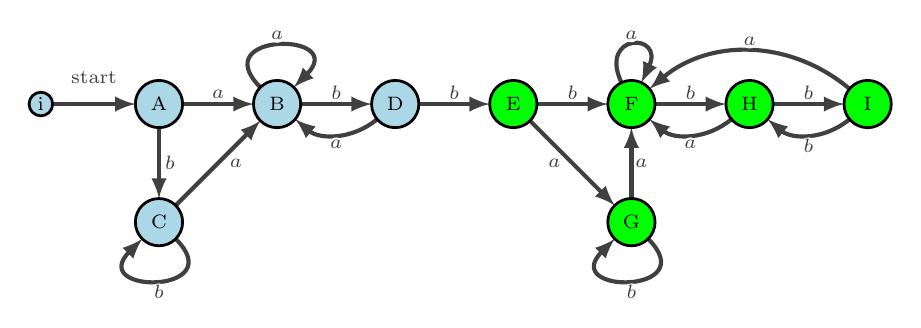
\begin{tikzpicture}
		\Vertex[label = i, size = 0.3]{Start}
		\Vertex[label = A, x = 1.5]{A}
		\Vertex[label = C, x = 1.5, y = -1.5]{C}
		\Vertex[label = B, x = 3]{B}
		\Vertex[label = D, x = 4.5]{D}
		\Vertex[label = E, x = 6, color = green]{E}
		\Vertex[label = F, x = 7.5, color = green]{F}
		\Vertex[label = G, x = 7.5, y = -1.5, color = green]{G}
		\Vertex[label = H, x = 9, color = green]{H}
		\Vertex[label = I, x = 10.5, color = green]{I}
		\Edge[Direct, label = start, position = {above=0.01mm}](Start)(A)
		\Edge[Direct, label = $a$, position = above](A)(B)
		\Edge[Direct, label = $b$, position = right](A)(C)
		\Edge[Direct, label = $b$, position = below, loopposition = -90](C)(C)
		\Edge[Direct, label = $a$, position = {below, right=1mm}](C)(B)
		\Edge[Direct, label = $a$, position = above, loopposition = 90](B)(B)
		\Edge[Direct, label = $b$, position = above](B)(D)
		\Edge[Direct, label = $a$, position = below, bend = 40](D)(B)
		\Edge[Direct, label = $b$, position = above](D)(E)
		\Edge[Direct, label = $b$, position = above](E)(F)
		\Edge[Direct, label = $a$, position = {below, left=1mm}](E)(G)
		\Edge[Direct, label = $b$, position = below, loopposition = -90](G)(G)
		\Edge[Direct, label = $a$, position = right](G)(F)
		\Edge[Direct, label = $a$, position = above, loopposition = 90, loopshape = 50, loopsize = 20](F)(F)
		\Edge[Direct, label = $b$, position = above](F)(H)
		\Edge[Direct, label = $a$, position = below, bend = 40](H)(F)
		\Edge[Direct, label = $b$, position = above](H)(I)
		\Edge[Direct, label = $b$, position = below, bend = 40](I)(H)
		\Edge[Direct, label = $a$, position = above, bend = -40](I)(F)
	\end{tikzpicture}\newline
	初始时, 只分可接收状态组和不可接收状态组.\newline
	因为从状态$D$出发经字符$b$可到达可接收状态, 而从状态$A, B, C$出发经任意字符都不能达到可接收状态, 因此$D$与$A, B, C$都是可分辨的, 因此$D$单独成为一组状态.\newline
	同理:从状态$B$出发可以到达状态$D$(另一个组), 而从$A, C$出发经任意字符都不能达到$D$, 因此$B$与$A, C$也是可分辨的, 故$B$也单独成为一组状态.\newline
	最后, 因为$A, C$经字符$a$均到达$B$所在的状态组(就是$B$本身), 经字符$b$均到达$A, C$所在的状态组(就是$A, C$本身), 因此$A, C$是不可分辨的, 将$A, C$进行合并, 合并为$A$.\newline
	同理:可接收状态$E, F, G, H, I$之间也是不可分辨的, 故将这$5$个状态合并为$E$.
	最终可得到最简DFA:\newline
	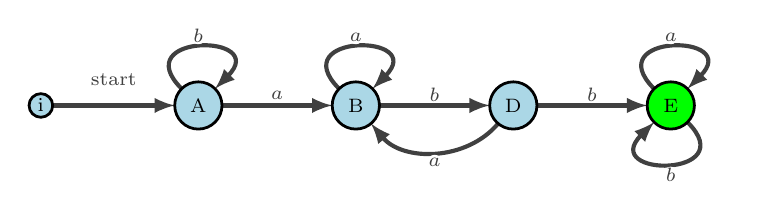
\begin{tikzpicture}
		\Vertex[label = i, size = 0.3]{Start}
		\Vertex[label = A, x = 2]{A}
		\Vertex[label = B, x = 4]{B}
		\Vertex[label = D, x = 6]{D}
		\Vertex[label = E, x = 8, color = green]{E}
		\Edge[Direct, label = start, position = above](Start)(A)
		\Edge[Direct, label = $b$, position = above, loopposition = 90](A)(A)
		\Edge[Direct, label = $a$, position = above](A)(B)
		\Edge[Direct, label = $a$, position = above, loopposition = 90](B)(B)
		\Edge[Direct, label = $b$, position = above](B)(D)
		\Edge[Direct, label = $a$, position = below, bend = 50](D)(B)
		\Edge[Direct, label = $b$, position = above](D)(E)
		\Edge[Direct, label = $a$, position = above, loopposition = 90](E)(E)
		\Edge[Direct, label = $b$, position = below, loopposition = -90](E)(E)
	\end{tikzpicture}
\end{document}









